\subsection{Title Classifier}
\label{sec:title}
%
%\begin{figure}
%\centering
%\epsfig{file=pic/PageTitle.eps,width=0.8\columnwidth}
%\caption{A Sample Top-K Like Title}
%\label{fig:title}
%\end{figure}

The title of a web page (string enclosed in {\tt<title>} tag) 
helps us identify a ``top-$k$'' page.
The goal of the classifier is to recognize ``top-$k$ like'' titles, 
the likely name of a ``top-$k$'' page. In general, 
a ``top-$k$ like'' title represents the topic of ``top-$k$'' list.
%Figure \ref{fig:title} shows a typical ``top-$k$ like'' title.
Note that a ``top-$k$ like'' title may contain multiple segments, and
usually only one segment describes the topic or concept of the list.

%Besides the features we mentioned in Section \ref{sec:intro} 
%(concept and number $k$),
%a ``top-$k$ like'' title could include some other elements;
%also as a web page, it may contain multiple segments, 
%among which only one segment is the main part.

%Therefore, the actual task for Title Classifier is 
%trying to recognize a proper number k with proper context in the title.
%If no such k is found, we consider the title not a ``top-$k$ like'' title.

%In our implementation, we build our classifier using a supervised machine-learning method.
We trained a Conditional Random Fields (CRF) \cite{CRFLafferty} model
from both positive and negative sample titles.
\cut{%%%%%%%%%%%%%%%%%
from 4000 negative titles (titles that contains a number but 
are not actually ``top-$k$ like'') and 2000 positives titles. The number $k$
is especially important because it serves as an anchor to a phrase that 
represent a ``top-$k$ like'' concept or topic.
We use \textit{word, lemma,} and \textit{POS tag} \cite{StanfordParser}
as the basic feature set.
Among these features, the number k is especially important for 
our system for the following reasons:
\begin{enumerate}
\item The number k is the common feature among all ``top-$k$ like'' titles, 
while other features may omit in some titles
\item The number k is indispensable for following components in our system: 
we need to extract a list with exact k items.
\item We can reduce our target page group to 
``those pages whose title contains at least one number''.
\end{enumerate}

Before we test an input title with the model we learned, 
%we need to transfer it to the format that our model can recognize
%(the same format for training data).
%Thus 
the following preprocessing steps are needed:

\begin{enumerate}
\item \textit{Normalizer}:
Fix some ill-formatted writing in the title and lowercase all the words.
\item \textit{Title Splitter}:
Split the title into segments by splitters such as ``|'' and ``-'', 
and select the longest one with a number as the main segment. 
\item \textit{Feature Generator}:
Generate mentioned features for each word in the main segment.
We use Stanford Parser \cite{StanfordParser} to get the lemma and POS tag features.
After this, we can get a table with words as rows and features as columns.
\end{enumerate}

After that, we can test the feature table of the input title. 
The model will label the number in the title with ``T'' or ``F'',
where ``T'' means the whole title is ``top-$k$ like''.
}%%%%%%%%%%%%%%%%%%%%
In addition to recognizing a ``top-$k$ like'' title, 
%the classifier need to provide information for the following components:
the classifier also transfers the cardinal digit word 
(word like ``ten'' or ``fifteen'') into the number $k$,
and outputs a set of Probase concepts such as 
``scientists'' which are mentioned in the title.

